\documentclass[conference]{IEEEtran}
\IEEEoverridecommandlockouts
% UT27 2-page extended abstract (500--1000 words + figures/tables).
% 빨간 글씨 = 그림/저자 정보 등 사용자가 채울 자리 표시.
\usepackage{cite}
\usepackage{amsmath,amssymb,amsfonts}
\usepackage{graphicx}
\usepackage{textcomp}
\usepackage{xcolor}
\newcommand{\todo}[1]{\textcolor{red}{[#1]}}
\def\BibTeX{{\rm B\kern-.05em{\sc i\kern-.025em b}\kern-.08em
    T\kern-.1667em\lower.7ex\hbox{E}\kern-.125emX}}
\begin{document}

\title{Formation Control of Unmanned Surface Vehicles with a Formation-Keeping Utility in Koopman-Based Optimal Control}

\author{\IEEEauthorblockN{\todo{1st Author Name}}
\IEEEauthorblockA{\textit{\todo{dept.}} \\
\textit{\todo{organization}}\\
\todo{City, Country} \\
\todo{email}}
\and
\IEEEauthorblockN{\todo{2nd Author Name}}
\IEEEauthorblockA{\textit{\todo{dept.}} \\
\textit{\todo{organization}}\\
\todo{City, Country} \\
\todo{email}}
\and
\IEEEauthorblockN{\todo{3rd Author Name}}
\IEEEauthorblockA{\textit{\todo{dept.}} \\
\textit{\todo{organization}}\\
\todo{City, Country} \\
\todo{email}}
}

\maketitle

\begin{abstract}
Coordinated formations of unmanned surface vehicles (USVs) can extend single-vehicle marine operations to cooperative survey and escort missions. A recent utility-function framework casts multi-robot navigation as optimal control of a Koopman-lifted system, where heterogeneous objectives are encoded as utility functions and the control input is obtained by linear programming at every step. The published framework, however, provides no mechanism for formation keeping: its only inter-robot term is a collision-avoidance penalty that monotonically favors separation. We introduce a formation-keeping utility term that peaks when the inter-vehicle distance equals a desired value, and show that it preserves the input-affine structure of the lifted dynamics, so the original identification and linear-programming pipeline is reused without modification. The extended framework is validated in two stages: numerical benchmarks, where the formation objective converges four orders of magnitude below its initial value with centimeter-level edge errors and no collisions while scaling to seven vehicles within real-time budgets, and a high-fidelity vessel-dynamics simulation with a leader platform and three follower USVs, where the formation holds a maximum edge error of 0.23 m over the evaluation window. The full paper will detail the formulation, the identifiability limits encountered, and an actuation-delay compensation that proved decisive under realistic vessel dynamics.
\end{abstract}

\begin{IEEEkeywords}
formation control, Koopman operator, unmanned surface vehicles, optimal control, linear programming
\end{IEEEkeywords}

\section{Introduction}
Underwater inspection and intervention increasingly depend on surface support: unmanned surface vehicles (USVs) relay communication and positioning to underwater assets that cannot receive GNSS. A single support vehicle, however, provides only one vantage point---its coverage moves with it, and its loss interrupts the mission. A \emph{formation} of USVs addresses these limits structurally: holding a prescribed geometry provides a spatially distributed, mobile baseline for surface-assisted localization and communication over an underwater work site, extends sensing coverage beyond one hull, and adds redundancy against single-vehicle failure. The value of the formation lies precisely in \emph{keeping} its geometry while moving---which makes formation keeping, not mere flocking, the control problem of interest.

Among data-driven approaches to multi-robot navigation, Zhao and Tao~\cite{tao2023merged} proposed an optimal-control framework in which navigation objectives---goal reaching, cruise speed, and collision avoidance---are encoded as utility functions, the joint robot state is lifted into a Koopman observable space, the lifted dynamics are approximated by a bilinear model, and the control input maximizing the one-step utility increase is obtained by a linear program (LP) at every step. Related Koopman treatments of multi-robot coordination address formation prediction~\cite{wang2022koopman} and game-theoretic guidance~\cite{zhao2023stackelberg}, but none combines utility-function encoding with LP-based optimal control for formation keeping: in~\cite{tao2023merged} the only inter-robot utility is a repulsive collision term, which cannot hold a formation shape.

This work extends the framework with a \emph{formation-keeping utility} and validates the extension through a staged simulation campaign, from numerical benchmarks to high-fidelity vessel dynamics, as a step toward field deployment on our USV platforms.

\todo{FIGURE 1 HERE (author-drawn): system overview --- USV formation escorting/supporting an underwater work site; shows why the formation geometry matters (distributed baseline, coverage, redundancy).}

\section{Formation-Keeping Utility}

\todo{FIGURE 2 HERE (author-drawn): flowchart of the control pipeline --- utility functions (goal, cruise, collision, formation-keeping) $\rightarrow$ Koopman lifting $\rightarrow$ bilinear approximation $\rightarrow$ per-step LP $\rightarrow$ vehicle inputs.}

For robots $i$ and $j$ with planar center distance $\lVert r_{ij}\rVert$, we define
\begin{equation}
\varphi^{(7)}_i(X)=\textstyle\sum_{j:(i,j)\in E}\exp\!\big(-(\lVert r_{ij}\rVert-d^{*}_{ij})^{2}/\sigma^{2}\big),
\end{equation}
a Gaussian that peaks at the desired spacing $d^{*}_{ij}$ over the formation edge set $E$. Unlike the collision term, which acts on surface clearance and only repels, the new term shapes the distance toward $d^{*}_{ij}$; collision safety remains delegated to the original term, giving a clean division of labor. Because the term depends on positions only, the same second-order expansion used for the original utilities applies, the lifted dynamics remain input-affine, and the LP formulation carries over verbatim---the formal basis of our pipeline-reuse claim. Followers are controlled in leader-relative coordinates, so the formation tracks a moving leader without re-deriving operating points.

Two findings from reproducing the base framework inform the full paper: (i) with only the published settings, data-driven bilinear identification is structurally underdetermined (parameter dimension far exceeding sample rank), consistent with the geometry-preservation concerns raised for bilinear Koopman models of nonholonomic robots~\cite{rosenfelder2024data}, motivating an analytic-gradient arm for control; and (ii) the published cruise-speed setting is scale-inconsistent with the collision-avoidance reaction distance and induces long-horizon collisions, which we resolve by parameterizing the cruise speed.

\section{Simulation Validation}
\subsection{Numerical benchmarks}
In double-integrator benchmarks with three robots (Fig.~\ref{fig:numeric}), the formation objective decreases from 151.4 to $1.9\times10^{-4}$ (baseline without the new term: 6.10), final edge errors are at most 0.013 m (baseline: up to 1.94 m), the run is collision-free, and the accumulated objective is lower than the baseline. At the desired spacing no conflict between the collision and formation terms is observed. The formulation scales to $N{=}3/5/7$ robots with per-step LP times of about 0.8/1.4/2.7 ms, an 18--62$\times$ margin against a 50 ms real-time budget.

\begin{figure}[t]
\centering
\begin{minipage}[b]{0.48\columnwidth}
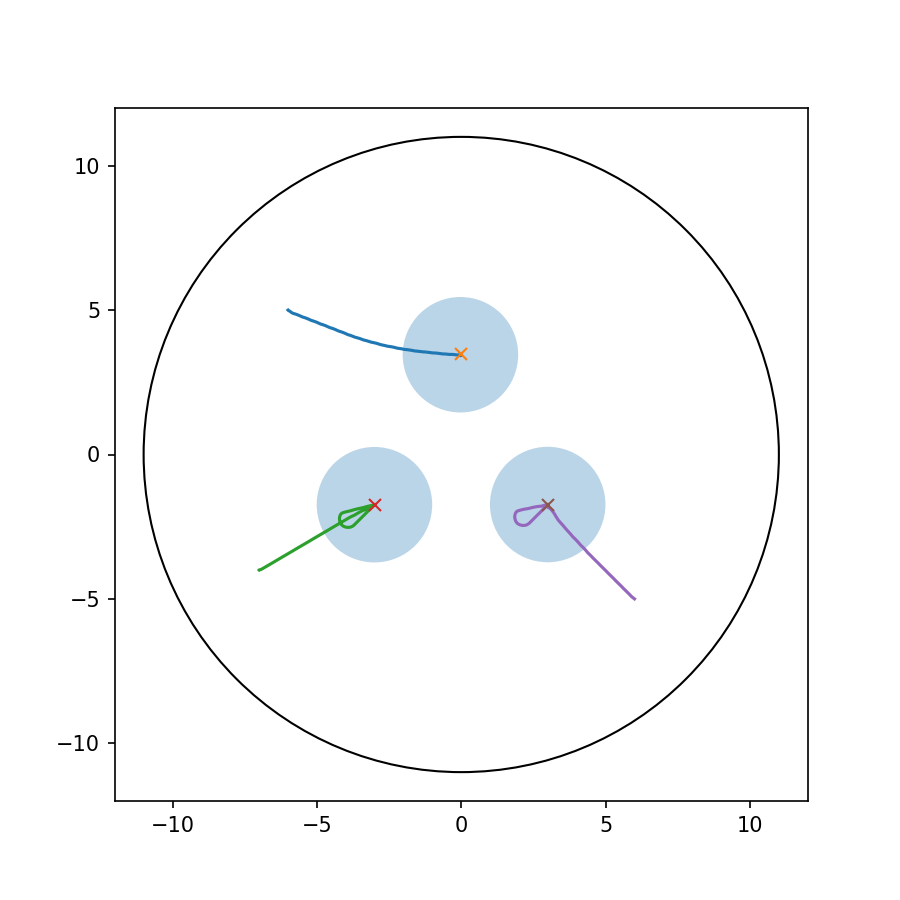
\includegraphics[width=\linewidth]{fig/e2_traj_phi7.png}
\centerline{\footnotesize (a)}
\end{minipage}\hfill
\begin{minipage}[b]{0.50\columnwidth}
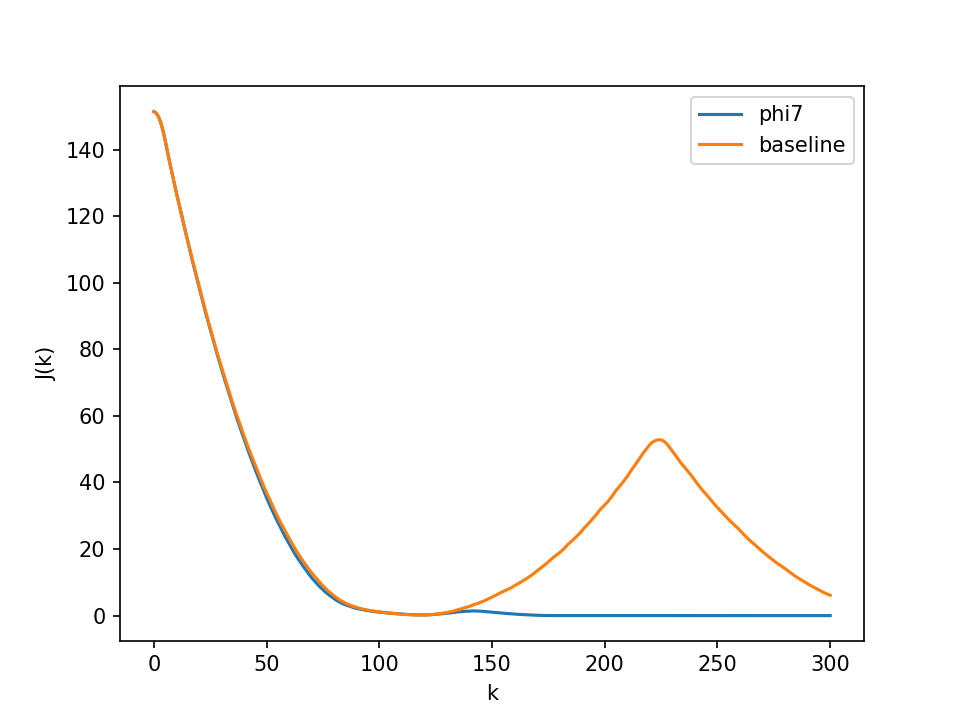
\includegraphics[width=\linewidth]{fig/e2_objective.png}
\centerline{\footnotesize (b)}
\end{minipage}
\caption{Numerical benchmark with three robots: (a) trajectories converging from scattered starts to the desired triangular formation (shaded circles: target regions); (b) formation objective over time---with the formation-keeping term the objective converges to near zero, whereas the baseline without it rebounds.}
\label{fig:numeric}
\end{figure}

\subsection{High-fidelity vessel dynamics}
The pipeline is then ported to a Stonefish simulation with full vessel hydrodynamics (buoyancy, drag, thruster dynamics): one leader platform and three follower USVs (Fig.~\ref{fig:stonefish}) in a hierarchical architecture (utility LP $\rightarrow$ velocity loop $\rightarrow$ thruster mixer). Online bilinear identification by recursive least squares succeeds in this layered setting, and the formation gate passes with a maximum edge error of 0.233 m over the final 30 s (criterion: 0.3 m), a median error of 0.024 m, and no collisions. Two negative results are preserved for the full paper: the identification-model control arm diverges under realistic dynamics (edge errors of 54--147 m), echoing~\cite{rosenfelder2024data}, and an actuation delay of 0.16 s---measured by input--acceleration cross-correlation---induces a relay-type limit cycle that is removed by delay-compensated state prediction, which proved decisive for passing the gate.

\begin{figure}[t]
\centering
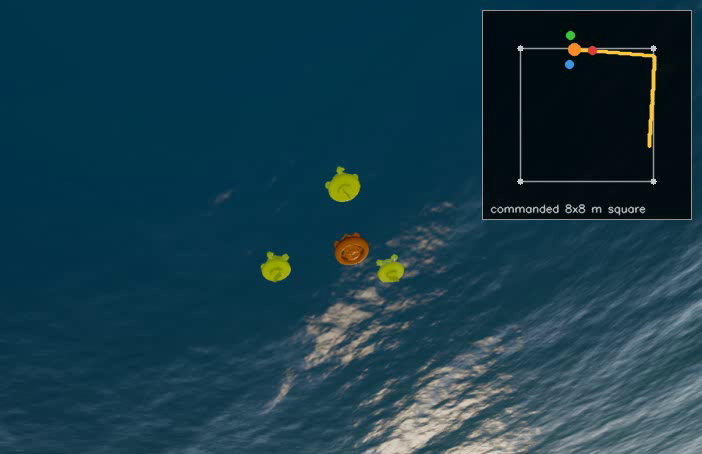
\includegraphics[width=0.92\columnwidth]{fig/stonefish_formation.png}
\caption{Stonefish high-fidelity simulation: the leader platform (orange) and three follower USVs (yellow) hold a triangular formation while the leader traverses a commanded square path (inset).}
\label{fig:stonefish}
\end{figure}

\todo{TABLE I HERE (optional): gate summary --- numerical benchmarks (objective decrease, edge errors, collision-free, N=3/5/7 control time) and Stonefish (max/median edge error) in one table. May be dropped if redundant with the text.}

\section{Conclusion}
A formation-keeping utility extends the utility-function Koopman optimal-control framework to multi-USV formation driving while reusing its identification and LP machinery unchanged. The staged campaign---numerical gates through high-fidelity vessel dynamics---supports the extension and surfaces deployment-relevant findings on identifiability and actuation delay. Integration with underwater-target following and field experiments on our USV fleet are ongoing and will be reported in the full paper.

\begin{thebibliography}{00}
\bibitem{tao2023merged} Q. Zhao and G. Tao, ``Koopman system approximation-based optimal control of multiple mobile robots,'' \emph{IEEE Trans. Control Syst. Technol.}, vol. 33, no. 3, pp. 963--979, 2025.
\bibitem{wang2022koopman} Y. Wang, T. Baba, and T. Hikihara, ``Robot formation control in nonlinear manifold using Koopman operator theory,'' \emph{Nonlinear Theory Appl., IEICE}, vol. 15, no. 2, pp. 501--517, 2024.
\bibitem{zhao2023stackelberg} Y. Zhao and Q. Zhu, ``Stackelberg game-theoretic trajectory guidance for multi-robot systems with Koopman operator,'' in \emph{Proc. IEEE Int. Conf. Robot. Autom. (ICRA)}, 2024.
\bibitem{rosenfelder2024data} M. Rosenfelder, L. Bold, H. Eschmann, P. Eberhard, K. Worthmann, and H. Ebel, ``Data-driven predictive control of nonholonomic robots based on a bilinear Koopman realization: Data does not replace geometry,'' \emph{Robot. Auton. Syst.}, vol. 194, p. 105156, 2025.
\end{thebibliography}

\end{document}
